\section{The Bias Persists Across Competence}
\label{sec:emergence}

If the canonical-prior bias were a symptom of undertraining, it should weaken as the policy improves. We test this by running a reduced reach-field ($50$\,mm, $4$ directions, $250$ rollouts) at four points along the full action-expert training trajectory ($10$k, $40$k, $70$k, $100$k steps), recovering both axes from each run: clean success (competence) and the clean-conditioned bias $\cossim(\ev,-\dv)$.

\paragraph{Bias is stable across the checkpoint ladder.} Across this full action-expert ladder, as clean success rises from $60\%$ to $74\%$, the bias stays flat, $\cossim(\ev,-\dv)\in[0.76,0.82]$, with the closer-to-canonical fraction in $[68\%,74\%]$ (\cref{fig:ladder}; per-checkpoint values in \cref{tab:ladder}). More training does not erode the bias---if anything it is marginally lower at the most competent checkpoint, within noise. The mislocalization is therefore stable as this policy becomes more competent over the measured range, not a transient artifact that more training within this trajectory removes.

\begin{figure}[t]
\centering
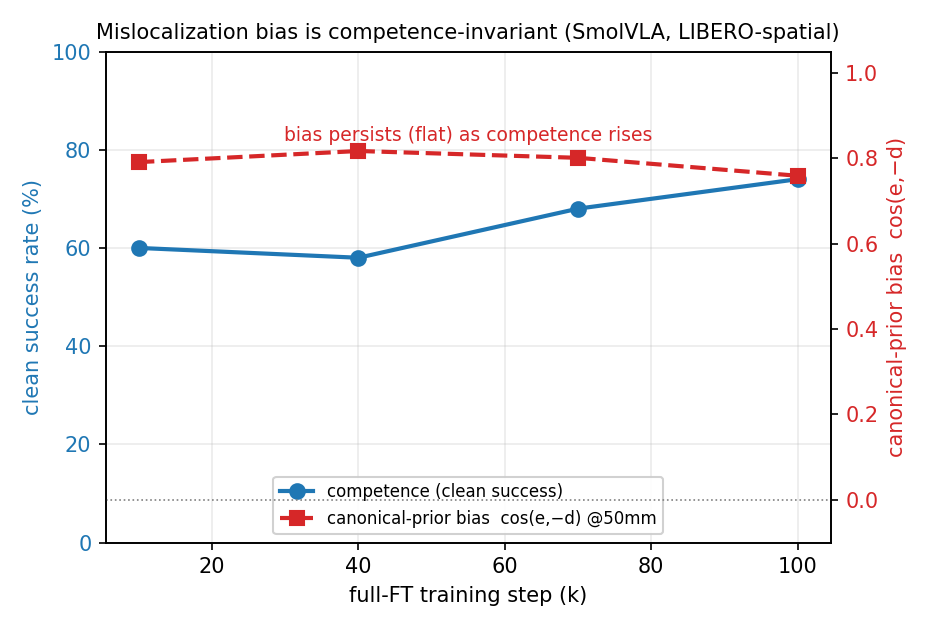
\includegraphics[width=0.55\textwidth]{figures/fig_ladder.png}
\caption{\textbf{Bias vs.\ competence along training.} As clean success rises ($60\!\to\!74\%$, blue), the canonical-prior bias $\cossim(\ev,-\dv)$ stays flat ($\sim\!0.78$, red). The failure mode does not diminish with competence.}
\label{fig:ladder}
\end{figure}

\begin{table}[t]
\centering
\caption{Emergence ladder (full action-expert checkpoints, $50$\,mm, clean-conditioned).}
\label{tab:ladder}
\small
\begin{tabular}{@{}lcccc@{}}
\toprule
Checkpoint & FT-10k & FT-40k & FT-70k & FT-100k \\
\midrule
Competence (clean success) & $60\%$ & $58\%$ & $68\%$ & $74\%$ \\
Bias $\cossim(\ev,-\dv)$ & $0.79$ & $0.82$ & $0.80$ & $0.76$ \\
Closer-to-canonical & $72\%$ & $74\%$ & $71\%$ & $68\%$ \\
\bottomrule
\end{tabular}
\end{table}

\paragraph{Caveat.} The competence range here is compressed: full action-expert fine-tuning is already $60\%$ competent by $10$k steps, so this ladder cannot probe the very-low-competence regime within the same recipe. We read it as evidence that the bias does not vanish as a competent policy gets \emph{more} competent, not as a claim about the full $0\!\to\!100\%$ competence axis (which would require mixing recipes and thereby confound competence with optimization).

\section{Generalization to a Second Suite}
\label{sec:generalization}

To test whether the canonical-prior reach is specific to LIBERO-spatial, we repeat the core protocol on \textbf{LIBERO-object}: a separate full action-expert checkpoint (same recipe, $68\%$ clean success), the E1r reach-field at $50$\,mm, and the E2 paste conditions (\cref{tab:suites}). Both findings replicate, and more strongly. The reach-field bias is sharper (median $\cossim(\ev,-\dv)=0.971$, $91\%$ of endpoints closer to canonical, vs.\ $0.759$/$68\%$ on spatial)---consistent with LIBERO-object's canonical object positions being tightly fixed across seeds, so the memorized reach target is sharper. The dissociation is also starker: showing the object displaced barely changes success (CT $79\%$ vs.\ CC $71\%$), but physically displacing it while showing it at canonical collapses success to $3\%$ (TC), with a null endpoint-steering coefficient ($S_{CT}=0.00$). The canonical-prior reach, and its decoupling from local visual object position, is therefore not specific to one LIBERO suite.

\begin{table}[t]
\centering
\caption{The canonical-prior reach and its visual decoupling replicate across two LIBERO suites.}
\label{tab:suites}
\small
\begin{tabular}{@{}lcc@{}}
\toprule
 & LIBERO-spatial & LIBERO-object \\
\midrule
Clean success (competence) & $74\%$ & $68\%$ \\
E1r $50$\,mm clean-cond.\ median $\cossim(\ev,-\dv)$ & $0.759$ $[0.69,0.85]$ & $0.971$ $[0.91,0.98]$ \\
\quad closer-to-canonical & $68\%$ & $91\%$ \\
E2 success: CC / CT / TC & $75 / 72 / 30\%$ & $71 / 79 / 3\%$ \\
\bottomrule
\end{tabular}
\end{table}
